\chapter{外文资料的调研阅读报告或书面翻译}

\title{将机器人抓取闭环:一种实时、生成的抓取合成方法}

{\heiti 摘要:} 本文提出了一种实时的、与对象无关的抓取合成方法,可用于闭环抓取。我们提出的生成抓取卷积神经网络 (GG-CNN) 预测每个像素的抓取质量和姿势。这种来自深度图像的一对一映射克服了当前深度学习抓取技术的局限性,避免了抓取候选的离散采样和较长的计算时间。此外,我们的 GG-CNN 在检测稳定抓取的同时具有与当前最先进技术相当的性能,并且数量级更小。我们的 GG-CNN 的轻量级和单通道生成特性允许以高达 50Hz 的频率进行闭环控制,从而在物体移动的非静态环境中以及机器人控制不准确的情况下实现准确抓取。在我们的真实世界测试中,我们在一组先前未见过的具有对抗性几何形状的物体上实现了 83\% 的抓取成功率,在抓取尝试期间移动的一组家用物体上实现了 88\% 的抓取成功率。在动态杂波中抓取时,我们也达到了 81\% 的准确率。

\section{引言}
为了在现实世界的非结构化环境中执行抓取和操作任务,机器人必须能够计算它可能遇到的几乎无限数量的物体的抓取。此外,它还需要能够在动态环境中发挥作用,无论是机器人工作空间的变化、感知的噪声和错误、机器人控制的不准确,还是机器人本身的扰动。


机器人抓取已经研究了几十年,产生了大量不同的技术。最近,深度学习技术在未知项目的抓取合成方面取得了一些最大的进步。这些方法允许学习与超出人工设计特征能力的高质量抓取相对应的特征。


但是,这些方法通常使用为对象识别而设计的卷积神经网络 (CNN) 架构的改编版本 ,并且在大多数情况下,单独对抓取候选对象进行采样和排序 ,导致计算时间较长大约一秒 到几十秒。因此,这些技术很少用于闭环抓取执行,并且依靠精确的相机校准和精确的机器人控制来成功抓取,即使在静态环境中也是如此。
\begin{figure}[h]
	\centering
	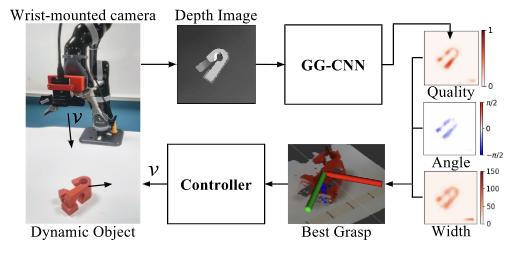
\includegraphics[width=0.8\textwidth]{附录/实时生成抓取管道}
	\caption{实时生成抓取管道。安装在机器人手腕上的摄像头捕捉包含要抓取的物体的深度图像。我们的生成抓取卷积神经网络 (GG-CNN) 为输入图像中的每个像素生成对映抓取——参数化为抓取质量、角度和抓取器宽度在几分之一秒内。计算最佳抓握并向机器人发出速度命令 ($v$)。闭环系统能够抓取动态对象并对控制做出反应。}
	\label{实时生成抓取管道}
\end{figure}


我们提出了一种不同的方法来为以前看不见的项目选择抓取点。我们的生成抓取卷积神经网络 (GG-CNN) 直接为输入深度图像中的每个像素生成对映抓取姿势和质量度量,并且对于动态环境中抓取的闭环控制来说足够快(图 1-1)。我们使用术语“生成”来区分我们的直接抓取生成方法和样本抓取候选的方法。


GG-CNN 相对于其他最先进的合成 CNN 的优势是双重的。首先,我们不依赖于抓取候选的采样,而是直接在像素基础上生成抓取姿势,类似于对象检测的进步,其中全卷积网络通常用于执行像素语义分割,而不是依赖于滑动窗口或边界框 [19]。其次,我们的 GG-CNN 的参数比其他用于抓取合成的 CNN 少几个数量级,这使得我们的抓取检测管道在配备 GPU 的台式计算机上只需 19 毫秒即可执行,速度足以进行闭环抓取。


我们在以下方面评估了我们系统的性能通过使用 Kinova Micorobot 对静态、动态和杂乱的物体进行抓取试验,实现不同的场景。在动态抓取试验中,在抓取尝试期间移动物体,我们在一组 8 个具有对抗几何的 3D 打印物体上实现了 83\% 的抓取成功率 [21],在从标准化对象集中选择的一组 12 个家居用品上实现了 88\% 的抓取成功率。此外,我们重现了 [32] 的动态杂波抓取实验,并显示抓取成功率提高了 81\%。当人为的误差被添加到机器人的控制中时,我们通过报告实验结果进一步说明使用闭环方法的优势。
\section{相关工作}
抓取未知物体抓取合成是指为给定物体制定稳定的机器人抓取方式,这是一个已经被广泛研究的主题,导致了大量的技术。从广义上讲,这些可以分为分析方法和经验方法。分析方法使用几何、运动学和动力学的数学和物理模型来计算稳定的抓取,但由于难以对机械手和对象之间的物理交互进行建模,因此往往不能很好地转移到现实世界中。


相比之下,经验方法侧重于使用模型和基于经验的方法。一些技术适用于已知项目,将良好的掌握点与对象模型或形状或熟悉的项目的离线数据库相关联,基于对象类或对象部分,但无法推广到新对象。


在抓取未知物体方面,最近随着基于视觉的深度学习技术的普及,取得了巨大的进步。许多这些技术共享一个共同的流程:对从图像或点云中采样的抓取候选者进行分类,然后使用卷积神经网络 (CNN) 对它们进行单独排序。一旦确定了最佳抓取候选者,机器人就会执行抓取开环(无需任何反馈),这需要相机和机器人之间的精确校准,机器人的精确控制和完全静态的环境。执行时间是抓取开环执行的主要原因。


在许多情况下,深度学习方法使用具有数百万个参数的大型神经网络 并使用滑动窗口以离散的偏移和旋转间隔处理抓取候选者,这在计算上是昂贵的,并且会导致抓取规划时间大约为一秒到几十秒。

一些方法通过预处理和修剪抓取候选者或同时预测一组离散的抓取候选者的质量来减少执行时间,在执行时间与采样的抓取数量之间进行权衡,但是忽略一些潜在的把握。


与我们的方法类似,Varley 等人,使用神经网络为图像中的手指放置生成像素级热图,但仍然依赖抓取规划器来确定最终的抓取姿势。


我们通过直接同时为图像中的每个像素生成抓取姿势来解决执行时间和抓取采样的问题,使用相对较小的神经网络。


闭环抓取使用视觉反馈将机器人闭环控制到所需姿势通常称为视觉伺服。视觉伺服方法的优点是它们能够适应动态环境并且不一定需要完全精确的相机校准或位置控制。许多工作将视觉伺服直接应用于抓取应用。然而,视觉伺服方法的性质意味着它们通常依赖于手工制作的图像特征来进行对象检测或对象姿态估计,因此不执行任何在线抓取合成,而是收敛到预先确定的目标姿势,并且不适用于未知对象。


最近有人提出基于 CNN 的抓取控制器将深度学习与闭环抓取相结合。两个系统都不是明确地执行抓取合成,而是学习控制器,这些控制器将潜在的控制命令映射到执行控制后的预期质量或距离,需要在每个时间步对许多潜在的命令进行采样。在这两种情况下,控制都以不超过大约 5Hz 的频率执行。虽然两者都是闭环控制器,但动态场景中的抓取仅在一项工作中提出中提出,我们重现了这些实验。


机器人抓取的基准测试由于使用的抓取检测技术范围广泛、对象集之间缺乏标准化以及不同物理硬件(例如机械臂、抓手或相机。许多人报告了对“家庭”对象集的抓取成功率,这些对象在使用的对象的数量和类型上差异很大。

ACRV Picking Benchmark (APB)和 YCBObject Set定义了项目集和操作任务,但在诸如仓库订单履行 (APB) 等任务上进行了基准测试或表格设置和块堆叠 (YCB),而不是通常报告的原始抓取成功率。此外,这两组中的许多项目对于许多机器人和抓手来说都是不切实际的小、大或重,因此尚未广泛用于机器人抓取实验。我们提出了一组 20 个可重复的测试项目,包括 8 个 3D 打印对抗来自的对象和来自 APB 和 YCB 对象集的 12 个项目,它们提供了足够广泛的尺寸、形状和难度,以有效地比较结果,同时不排除任何常见机器人、夹具或相机的使用。

\section{总结}
我们展示了我们的生成抓取卷积神经网络 (GG-CNN),这是一种与对象无关的抓取合成模型,它直接从深度图像以像素为单位生成抓取姿势,而不是像其他深度学习技术那样对单个抓取候选对象进行采样和分类。我们的 GG-CNN 比其他最近的抓取网络小几个数量级,使我们能够以高达 50Hz 的速率生成抓取并执行闭环控制。我们通过抓取试验表明我们的系统能够获得最先进的技术导致抓取未知的动态对象,包括动态杂波中的对象。此外,在存在模拟机器人控制错误的情况下,我们的闭环抓取方法明显优于开环方法。我们通过使用两个标准对象集(一组具有对抗几何的八个 3D 打印对象)来鼓励机器人抓取实验的可重复性。 21]加上来自标准机器人基准对象集的十二个家居用品的建议集,并通过定义我们的动态抓取实验的参数。在我们的两个对象集上,当对象在抓取尝试期间移动时,抓取成功率分别为 83\% 和 88\%,而动态杂波中的对象抓取成功率为 81\%。